\documentclass[tikz]{standalone}
\usepackage[dvipsnames]{xcolor}
\usepackage{tikz}
\usetikzlibrary{calc}

\begin{document}
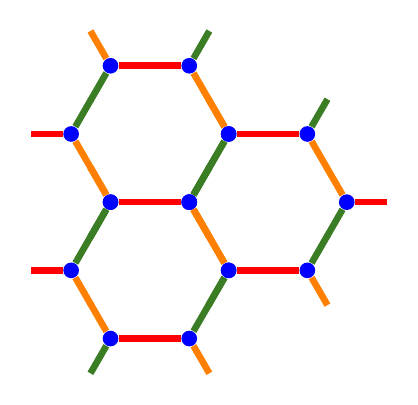
\begin{tikzpicture}[scale=1, baseline=(current bounding box.center)]
  \pgfmathsetmacro{\s}{1}              % bond length
  \pgfmathsetmacro{\h}{0.86602540378*\s} % sqrt(3)/2 * s

  \tikzset{
    hc node/.style={circle, fill=blue, inner sep=2pt},
    red bond/.style={red, line width=2.4pt},
    green bond/.style={OliveGreen, line width=2.4pt},
    orange bond/.style={orange, line width=2.4pt},
  }

  \newcommand{\drawhexAsite}[2]{
    \node[hc node] (H#1A) at ($ #2 + (-0.5*\s,0) $) {};
    \draw[red bond]    (H#1A) -- +(   0:0.51*\s) ;
    \draw[orange bond] (H#1A) -- +(+120:0.51*\s) ;
    \draw[green bond]  (H#1A) -- +(-120:0.51*\s) ;
  }
  \newcommand{\drawhexBsite}[2]{
    \node[hc node] (H#1B) at ($ #2 + (+0.5*\s,0) $) {};
    \draw[red bond]    (H#1B) -- +( 180:0.51*\s) ;
    \draw[orange bond] (H#1B) -- +(- 60:0.51*\s) ;
    \draw[green bond]  (H#1B) -- +(+ 60:0.51*\s) ;
  }
  \newcommand{\drawhexABbond}[2]{
    \drawhexAsite{#1}{#2};
    \drawhexBsite{#1}{#2};
  }
  \newcommand{\drawhexagon}[2]{
    \drawhexABbond{#1top}{#2 + (0,\h)};
    \drawhexABbond{#1bot}{#2 + (0,-\h)};
    \drawhexAsite{#1R}{#2 + (+1.5,0)};
    \drawhexBsite{#1L}{#2 + (-1.5,0)};
  }

  % Three-hex cluster
  \drawhexagon{C1}{(0,+\h)};
  \drawhexagon{C2}{(0,-\h)};
  \drawhexagon{C3}{(1.5,0)};
\end{tikzpicture}
\end{document}
